\documentclass[12pt,aspectratio=169]{beamer}
\usetheme{Copenhagen}
\usecolortheme{whale}
\setbeamertemplate{navigation symbols}{}
\setbeamertemplate{footline}[frame number]
\usepackage{amsmath,amssymb}
\usepackage{tikz}
\usepackage{booktabs}
\usepackage{listings}
\usepackage{xeCJK}
\setCJKmainfont{Noto Serif CJK SC}
\setCJKsansfont{Noto Sans CJK SC}
\setCJKmonofont{Noto Sans CJK SC}

\lstset{
  basicstyle=\ttfamily\footnotesize,
  keywordstyle=\color{blue}\bfseries,
  commentstyle=\color{gray},
  showstringspaces=false,
  numbers=left,
  numberstyle=\tiny\color{gray},
  frame=single,
  tabsize=4,
  language=C
}

\title{数值计算中的人工智能角色}
\subtitle{以高斯消去法与 LU 分解为例}
\author{Crazyfish}
\date{\today}

\begin{document}

% ==================== frame 1: 标题 ====================
\begin{frame}
\titlepage
\end{frame}

% ==================== frame 2: 背景 ====================
\begin{frame}[shrink]{高斯消去法与 LU 分解}
\framesubtitle{从线性方程组到矩阵分解}

\small
\[
A\mathbf{x}=\mathbf{b},\qquad
A = \begin{pmatrix}
a_{11} & a_{12} & a_{13}\\
a_{21} & a_{22} & a_{23}\\
a_{31} & a_{32} & a_{33}
\end{pmatrix},\;
\mathbf{b} = \begin{pmatrix}b_1\\b_2\\b_3\end{pmatrix}
\]

\vspace{4pt}
\begin{columns}[T]
\column{0.5\textwidth}
\textbf{高斯消去法：} 初等行变换 $\to$ 上三角 $\to$ 回代求解。

\begin{itemize}
  \item 第 $k$ 步：用主元行消去下方第 $k$ 列
  \item 乘子 $m_{ik} = a_{ik}/a_{kk}$
  \item $a_{ij} \leftarrow a_{ij} - m_{ik}\cdot a_{kj}$
\end{itemize}

\column{0.5\textwidth}
\textbf{LU 分解：} 消去过程的乘子构成单位下三角矩阵 $L$。
\[
A = LU,\quad
L = \begin{pmatrix}1&0&0\\m_{21}&1&0\\m_{31}&m_{32}&1\end{pmatrix}
\]

\vspace{4pt}
选主元后 $PA = LU$。求解步骤：\\
分解 ($O(\frac{2}{3}n^3)$) $\to$ 前代 $L\mathbf{y}=P\mathbf{b}$ $\to$ 回代 $U\mathbf{x}=\mathbf{y}$。
\end{columns}
\end{frame}

% ==================== frame 3: 复杂度 ====================
\begin{frame}[shrink]{算法结构与计算复杂度}

\begin{columns}[T]
\column{0.45\textwidth}
\small
\textbf{kij 右看 LU (选主元):}

\vspace{2pt}
\footnotesize
对 $k=0,\dots,n-1$:
\begin{enumerate}
  \item 列主元：找 $p$ 使 $|a_{pk}|$ 最大，必要时交换行
  \item 乘子: $a_{ik} \leftarrow a_{ik}/a_{kk}$ \quad ($i>k$)
  \item rank-1 更新: $a_{ij} \leftarrow a_{ij} - a_{ik}\cdot a_{kj}$
\end{enumerate}

\column{0.55\textwidth}
\renewcommand{\arraystretch}{1.2}
\begin{tabular}{@{}lcc@{}}
\toprule
\textbf{阶段} & \textbf{flops} & \textbf{主导项} \\
\midrule
LU 分解 & $\frac{2}{3}n^3$ & $n^3$ \\
前代/回代 & $n^2$ & $n^2$ \\
列主元搜索 & $\frac{1}{2}n^2$ & $n^2$ \\
\bottomrule
\end{tabular}

\vspace{4pt}
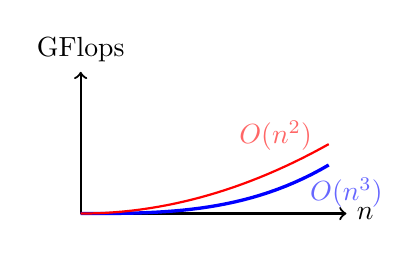
\begin{tikzpicture}[scale=0.45]
  \draw[->, thick] (0,0) -- (7.5,0) node[right] {$n$};
  \draw[->, thick] (0,0) -- (0,4) node[above] {GFlops};
  \draw[blue, very thick, domain=0:7, samples=30]
    plot (\x, {0.004 * \x * \x * \x});
  \draw[red, thick, domain=0:7, samples=30]
    plot (\x, {0.04 * \x * \x});
  \node[blue!60] at (7.5,0.6) {$O(n^3)$};
  \node[red!60] at (5.5,2.2) {$O(n^2)$};
\end{tikzpicture}
\end{columns}

\vspace{2pt}
$n$ 较大时 $O(n^3)$ 消去阶段完全主导。所有优化必须集中于此。
\end{frame}

% ==================== frame 4: 六重挑战 ====================
\begin{frame}[shrink]{从教科书到高性能代码的技术挑战}

教科书上的伪代码 15 行。生产级实现需要跨越六个技术层次：

\vspace{4pt}
\begin{columns}[T]
\column{0.5\textwidth}
\begin{enumerate}
  \item \textbf{数值稳定性}
  \begin{itemize}
    \item 零主元导致除零；小主元放大舍入误差
    \item 列主元保证乘子有界 ($|m_{ik}|\le 1$)
  \end{itemize}
  \item \textbf{数据结构}
  \begin{itemize}
    \item row-major vs column-major
    \item 原位覆盖：L 的严格下三角与 U 共存于 A
  \end{itemize}
  \item \textbf{Cache / 内存层次}
  \begin{itemize}
    \item $n=2000$ 矩阵 $\sim$32MB，远超 L3
    \item 朴素 kij 循环 $\to$ 每次迭代 cache miss
    \item 分块 (blocking) 将工作集控制在 cache 内
  \end{itemize}
\end{enumerate}

\column{0.5\textwidth}
\begin{enumerate}
  \setcounter{enumi}{3}
  \item \textbf{SIMD 向量化}
  \begin{itemize}
    \item 编译器自动向量化远不如手工调优
    \item AVX-512: 单指令 8 个 double；FMA 单周期乘加
  \end{itemize}
  \item \textbf{多核并行}
  \begin{itemize}
    \item 面板分解 (panel LU) 存在数据依赖
    \item OpenMP 行间并行 + nowait 减少同步开销
  \end{itemize}
  \item \textbf{GPU 加速}
  \begin{itemize}
    \item 不同的内存模型与编程范式
    \item 批量 LU 在 cuSOLVER 中；数据传输需与计算重叠
  \end{itemize}
\end{enumerate}
\end{columns}

\vspace{4pt}
\begin{center}
\textbf{每一层都需要专门的领域知识，远超数值方法课程的范围。}
\end{center}
\end{frame}

% ==================== frame 5: 分块LU ====================
\begin{frame}[shrink]{一个实现技术困难的例子：分块 LU 的实际实现}

\textbf{分块右看 LU (Blocked Right-Looking):}

\small
\begin{enumerate}
  \item \textbf{Panel LU:} 对列块 $A[k:n,\,k:k+kb]$ 做无分块 LU，选主元并交换整行
  \item \textbf{dtrsm:} $L_{\text{top}}\cdot X = A_{\text{top\_right}}$ — 多右端三角求解
  \item \textbf{dgemm:} $A_{\text{bot\_right}} \mathrel{-}= A_{\text{bot\_left}}\cdot U_{\text{right}}$ — 矩阵乘 (占 $>90\%$ 计算)
\end{enumerate}

\vspace{6pt}
\textbf{关键设计决策：}

\begin{columns}[T]
\column{0.5\textwidth}
\begin{itemize}
  \item \textbf{块大小 nb=128：} panel + dgemm 工作集 $\sim$2MB，适配 L2/L3
  \item \textbf{s-i-j 循环序：} 最内层 $B[s][:]$ 和 $C[i][:]$ 均 stride-1
  \item \textbf{自适应回落：} $n<500$ 走原始无分块路径
\end{itemize}

\column{0.5\textwidth}
\begin{itemize}
  \item \textbf{OpenMP 策略：} 外层分 $s$ 方向，nowait 消除 barrier
  \item \textbf{阈值并行：} dgemm flops $>50$M 才启用 OpenMP
  \item \textbf{面板分解：} 仍为串行，占总计算量 $\sim O(n^2)$
\end{itemize}
\end{columns}

\vspace{6pt}
\begin{center}
\footnotesize
\textbf{教科书：15 行伪代码。~~ \texttt{gauss\_opt.c}：230 行 C，含面板 + dtrsm + 并行 dgemm。}
\end{center}
\end{frame}

% ==================== frame 6: 二层生态 ====================
\begin{frame}[shrink]{数值计算的二层生态}
\framesubtitle{计算软件和计算库 — 传统计算应用的关键}

\small
\begin{center}
\renewcommand{\arraystretch}{1.3}
\begin{tabular}{@{}p{2.5cm} p{5cm} p{5cm}@{}}
\toprule
& \textbf{计算软件} & \textbf{计算库} \\
\midrule
\textbf{定位} & 高层交互环境，面向最终用户 & 底层性能引擎，面向开发者 \\
\textbf{代表} & Matlab, NumPy/SciPy & MKL, OpenBLAS, Eigen, LAPACK \\
\textbf{接口} & Win 窗口中的脚本/命令行 & C/Fortran API，手动内存管理 \\
\textbf{优势} & 易学易用，可视化、调试、I/O & 极致性能，硬件级调优 \\
\textbf{性能来源} & 内部调用计算库 & 手写编译 + 多级 tiling + SIMD \\
\bottomrule
\end{tabular}
\end{center}

\vspace{6pt}
\textbf{关系：} NumPy $\to$ OpenBLAS/MKL；Matlab $\to$ MKL；Eigen 纯头文件 + 可选 MKL 后端。

\vspace{2pt}
\textbf{选软件是选体验，选库是选性能。} 大多数最终用户通过软件间接使用库，不关心底层细节。
\end{frame}

% ==================== frame 7: 新论点 — 跨越计算软件 ====================
\begin{frame}[shrink]{跨越计算软件 — 一个新的实践范式}
\framesubtitle{学习/科研中，AI + 计算库 \,$\approx$\, 计算软件}

\small
\begin{columns}[T]
\column{0.5\textwidth}
\textbf{传统路径：} 用户 $\to$ \emph{计算软件} $\to$ 计算库

\vspace{2pt}
计算软件 \, = \, 计算库 \,+\, 易用封装层
\begin{itemize}
  \item 后端调用 (Fortran 接口、内存布局)
  \item 编译链接配置 (rpath、版本匹配)
  \item REPL / 笔记本 / 可视化
\end{itemize}

\column{0.5\textwidth}
\textbf{AI 时代的新路径：} 用户 \,+\, \emph{AI} \,$\to$ 计算库

\vspace{2pt}
AI 替代了"易用封装层"
\begin{itemize}
  \item AI 写库绑定代码 (\texttt{extern dgetrf\_}\,…)
  \item AI 配置编译链接 (\texttt{-lmkl\_rt})
  \item 用户自己掌控算法骨架与数据结构
\end{itemize}
\end{columns}

\vspace{6pt}
\begin{block}{核心论点}
在以\textbf{学习}和\textbf{科研}为目的的具体计算问题上，我们可以\textbf{跨越计算软件}，通过 AI 直接调用计算库，获得\textbf{不低于软件的效率}。
\end{block}

\vspace{2pt}
\textbf{为什么这一点过去做不到？} 直接调库的"绑定 + 配置"门槛过高，普通用户被劝退；为此付出代价才使用软件。\textbf{AI 让这个门槛归零。}
\end{frame}

% ==================== frame 8: 库的障碍 = AI 的价值 ====================
\begin{frame}[fragile,shrink]{使用计算库的真实障碍 = AI 的价值所在}

\textbf{直接使用 MKL / LAPACK 的若干门槛：}
\begin{itemize}
  \item Fortran 接口的名称修饰 (\texttt{dgetrf\_}) 与全指针传参
  \item 列主元 vs 行主元的存储转换 (LAPACK 默认列优先)
  \item Workspace 大小查询 (\texttt{lwork=-1}) 与 \texttt{ipiv} 数组管理
  \item 编译链接 (\texttt{-lmkl\_rt}, \texttt{-Wl,-rpath}, 版本匹配)
\end{itemize}

\vspace{4pt}
\textbf{AI 桥接的输出 — 60 行代码搞定一切：}

\begin{lstlisting}[language=C,basicstyle=\ttfamily\scriptsize,belowskip=-2pt,aboveskip=0pt,numbers=none]
extern void dgetrf_(int *m, int *n, double *a, int *lda,
                    int *ipiv, int *info);
extern void dgetrs_(char *trans, int *n, int *nrhs, double *a,
                    int *lda, int *ipiv, double *b, int *ldb, int *info);

/* 调用 — 只需 2 行 */
dgetrf_(&n, &n, A, &n, ipiv, &info);                /* LU 分解 */
dgetrs_(&trans, &n, &nrhs, A, &n, ipiv, b, &n, &info); /* 求解 */
\end{lstlisting}

\vspace{2pt}
\begin{block}{}
\small \textbf{这层 60 行的绑定代码，正是过去把普通用户挡在 MKL 外面的墙。AI 让这堵墙的成本归零。}
\end{block}
\end{frame}

% ==================== frame 9: 实验设计 ====================
\begin{frame}[shrink]{实验设计 — 四路对照 + 软件基线}

\textbf{核心比较：} AI 直接调库 (v3) vs 计算软件 (NumPy/SciPy)。

\vspace{4pt}
\footnotesize
\begin{center}
\renewcommand{\arraystretch}{1.2}
\begin{tabular}{@{}l p{4.3cm} p{4.7cm} p{1.6cm}@{}}
\toprule
\textbf{版本} & \textbf{向 AI 提出的要求} & \textbf{AI 交付内容} & \textbf{代码量} \\
\midrule
v1 原始 C   & 带列主元的高斯消去法 & kij 右看 + 选主元 + 回代 & $\sim$120 行 \\
v2 优化 C   & 分块 + OpenMP 并行 & 分块 LU + s-i-j dgemm & $\sim$230 行 \\
v3 AI+MKL   & 调用 MKL 的 dgetrf & Fortran 接口绑定 + 链接 & $\sim$60 行 \\
\textbf{基线} & NumPy.solve / SciPy.lu\_factor & 软件直接调用 (链 MKL) & 1 行 \\
\bottomrule
\end{tabular}
\end{center}
\normalsize

\vspace{4pt}
\small
\textbf{环境：} 16 核 x86\_64；gcc -O3 -march=native；双精度；$n=100$–$4000$。

\textbf{后端确认：} \texttt{numpy.show\_config()} $\Rightarrow$ \texttt{mkl-sdl 2023.1}，与 v3 链接同一份 MKL。

\vspace{4pt}
\begin{center}
\textbf{NumPy/SciPy 代表"计算软件"路径，v3 是"AI 跨越软件"路径 — 比较二者即为核心实验。}
\end{center}
\end{frame}

% ==================== frame 10: 版本一 ====================
\begin{frame}[fragile]{版本一：原始 C 实现 — kij 右看算法}
\framesubtitle{AI 生成的核心代码（gauss.c）}

\begin{lstlisting}[language=C,basicstyle=\ttfamily\scriptsize,belowskip=-2pt,numbers=none,aboveskip=0pt]
for (int k = 0; k < n - 1; k++) {
    /* 列主元 */
    int pivot = k;
    for (int i = k+1; i < n; i++)
        if (fabs(U[i*n+k]) > fabs(U[pivot*n+k])) pivot = i;
    if (fabs(U[pivot*n+k]) < 1e-15) return -1;
    if (pivot != k) { swap_rows(n, U, k, pivot); swap(&x[k], &x[pivot]); }

    /* 消去: rank-1 update */
    double *Uk = U + k*n, dk = Uk[k];
    for (int i = k+1; i < n; i++) {
        double f = U[i*n+k] / dk;
        U[i*n+k] = f;                     /* multiplier → L */
        for (int j = k+1; j < n; j++) U[i*n+j] -= f * Uk[j];
        x[i] -= f * x[k];
    }
}
/* 回代: x[i] = (x[i] - sum_{j>i} Uij*x[j]) / Uii */
\end{lstlisting}

\vspace{2pt}
\small
\textbf{教学代码：} kij 循环、列主元、restrict 指针、内存管理。\\
\textbf{这是为了学习而写 — 不是为了和库竞争。} $n>1000$ 时性能崩溃。
\end{frame}

% ==================== frame 10a: v1 头文件与库依赖 ====================
\begin{frame}[fragile]{版本一：头文件与库依赖}
\framesubtitle{标准 C 库 — 零安装成本}

\textbf{头文件 (gauss.c / test.c):}
\begin{lstlisting}[language=C,basicstyle=\ttfamily\footnotesize,belowskip=-2pt,aboveskip=0pt,numbers=none]
#include <stdio.h>      /* I/O               */
#include <stdlib.h>     /* malloc / free     */
#include <string.h>     /* memcpy            */
#include <math.h>       /* fabs, sqrt        */
#include <time.h>       /* clock_gettime     */
\end{lstlisting}

\vspace{4pt}
\footnotesize
\begin{columns}[T]
\column{0.5\textwidth}
\textbf{链接库与编译：}
\begin{itemize}\itemsep0pt
  \item \texttt{libc} — C 标准库 (自动)
  \item \texttt{libm} — 数学函数 (\texttt{-lm})
\end{itemize}
\begin{lstlisting}[basicstyle=\ttfamily\scriptsize,belowskip=-2pt,aboveskip=0pt,numbers=none]
gcc -O3 -march=native -o test \
    test.c gauss.o -lm
\end{lstlisting}

\column{0.5\textwidth}
\textbf{来源与许可：}
\begin{itemize}\itemsep0pt
  \item \textbf{GNU glibc} (libc, libm)
  \item LGPL — \textbf{完全开源}
  \item Linux 默认安装, 零配置
  \item 所有 POSIX 平台可用
  \item 零外部依赖, 最小基线
\end{itemize}
\end{columns}
\end{frame}

% ==================== frame 11: 版本二 ====================
\begin{frame}[fragile]{版本二：分块 LU + OpenMP — 结构与并行内核}
\framesubtitle{AI 生成的核心代码（gauss\_opt.c）}

\begin{lstlisting}[language=C,basicstyle=\ttfamily\scriptsize,belowskip=-2pt,numbers=none,aboveskip=0pt]
/* 顶层：面板分解 → dtrsm → dgemm */
for (int k = 0; k < n; k += nb) {
    int kb = (k+nb < n) ? nb : (n-k);
    panel_lu(n, A, k, kb, piv);
    if (k+kb < n) {
        dtrsm_lower(n, A, k, kb);
        dgemm_sij(n, A, k, kb);     /* 主要计算量, OMP 并行 */
    }
}
/* dgemm s-i-j 并行内核 (stride-1 内层 + SIMD) */
#pragma omp for schedule(static) nowait
for (int i = 0; i < m; i++) {
    #pragma omp simd
    for (int j = 0; j < p; j++)
        C[i*n+j] -= A_panel[i*n+s] * B_top[s*n + j];
}
\end{lstlisting}

\vspace{2pt}
\footnotesize
\textbf{通过 AI 在没有商业库时做到的极致：} 三层分块、s-i-j 序 stride-1、OMP 策略、阈值回落。
\textbf{v2 代表旧时代编程高手的极限，但仍然无法突破有硬件后门的商业库。}
\end{frame}

% ==================== frame 11a: v2 头文件与库依赖 ====================
\begin{frame}[fragile]{版本二：头文件与库依赖}
\framesubtitle{OpenMP — 随 GCC 自带的开源并行运行时}

\textbf{头文件 (gauss\_opt.c):}
\begin{lstlisting}[language=C,basicstyle=\ttfamily\footnotesize,belowskip=-2pt,aboveskip=0pt,numbers=none]
#include <stdio.h>      /* 同 v1                       */
#include <stdlib.h>
#include <string.h>
#include <math.h>
#include <omp.h>        /* OpenMP API: 并行/SIMD 指令  */
\end{lstlisting}

\vspace{4pt}
\footnotesize
\begin{columns}[T]
\column{0.5\textwidth}
\textbf{链接库与编译：}
\begin{itemize}\itemsep0pt
  \item \texttt{libgomp} — GCC OpenMP runtime
  \item \texttt{libpthread} — POSIX 线程 (自动)
  \item \texttt{-fopenmp} 自动链接
\end{itemize}
\begin{lstlisting}[basicstyle=\ttfamily\scriptsize,belowskip=-2pt,aboveskip=0pt,numbers=none]
gcc -O3 -march=native -fopenmp \
    -o test_opt test_opt.c \
    gauss_opt.o gauss.o -lm
\end{lstlisting}

\column{0.5\textwidth}
\textbf{来源与许可：}
\begin{itemize}\itemsep0pt
  \item \textbf{libgomp} (GCC OpenMP)
  \item GPL + linking exception — \textbf{开源}
  \item 随 GCC 安装, 无独立配置
  \item Linux / macOS / Windows 通用
  \item LLVM/Clang 用 \texttt{libomp} (等价)
\end{itemize}
\end{columns}
\end{frame}

% ==================== frame 12: 版本三 ====================
\begin{frame}[fragile]{版本三：AI+MKL 薄绑定层}
\framesubtitle{v3 = AI 把"软件路径"拆开，把里面的引擎装到你代码里}

\begin{lstlisting}[language=C,basicstyle=\ttfamily\footnotesize,belowskip=-2pt,numbers=none,aboveskip=0pt]
/* Fortran 接口声明 -- 无头文件, 跨版本兼容 */
extern void dgetrf_(int *m, int *n, double *a,
                    int *lda, int *ipiv, int *info);
extern void dgetrs_(char *trans, int *n, int *nrhs,
                    double *a, int *lda, int *ipiv,
                    double *b, int *ldb, int *info);

/* 调用 -- 仅 2 行, 全传指针 */
dgetrf_(&n, &n, A, &n, ipiv, &info);              /* LU 分解 */
dgetrs_(&trans, &n, &nrhs, A, &n, ipiv, x, &n, &info);
\end{lstlisting}

\vspace{4pt}
\small
\textbf{AI 处理了调用商业库所有复杂细节：} Fortran 名称修饰 (\texttt{dgetrf\_})、全指针传参、编译链接配置 (\texttt{-lmkl\_rt})。

\vspace{2pt}
\textbf{等价于 \texttt{np.linalg.solve(A,b)} 在内部所做的事情， 只是这次它在你的 C 代码里工作。（Matlab 也一样。）}
\end{frame}

% ==================== frame 12a: v3 头文件与库依赖 ====================
\begin{frame}[fragile,shrink]{版本三：头文件与库依赖}
\framesubtitle{Intel MKL 商业库 + 多种开源替代}

\textbf{头文件：} 零 MKL 头文件依赖 — 仅 \texttt{extern} Fortran 声明:
\begin{lstlisting}[language=C,basicstyle=\ttfamily\scriptsize,belowskip=-2pt,aboveskip=0pt,numbers=none]
extern void dgetrf_(int *m, int *n, double *a, int *lda, int *ipiv, int *info);
\end{lstlisting}

\vspace{4pt}
\footnotesize
\begin{center}
\renewcommand{\arraystretch}{1.1}
\setlength{\tabcolsep}{4pt}
\begin{tabular}{@{}l l l l@{}}
\toprule
\textbf{库} & \textbf{来源} & \textbf{许可} & \textbf{链接} \\
\midrule
\textbf{Intel MKL 2023.1} (本实验) & Intel oneAPI & 商业, 免费授权 & \texttt{-lmkl\_rt -ldl} \\
OpenBLAS 0.3.x         & GitHub/xianyi   & BSD-3, 开源 & \texttt{-lopenblas} \\
BLIS / LAPACK ref.     & FLAME / Netlib  & BSD, 开源    & \texttt{-lblis} / \texttt{-llapack} \\
Eigen 3.4              & MPL2 项目       & MPL2, 开源   & 纯头文件 (\texttt{-I}) \\
\bottomrule
\end{tabular}
\end{center}
\normalsize

\vspace{2pt}
\textbf{本实验编译命令：}
\begin{lstlisting}[basicstyle=\ttfamily\scriptsize,belowskip=-2pt,aboveskip=0pt,numbers=none]
gcc -O3 -fopenmp -o bench_mkl bench_mkl.c gauss.o gauss_opt.o \
    -L$(CONDA_PREFIX)/lib -Wl,-rpath,$(CONDA_PREFIX)/lib -lmkl_rt -lm -ldl
\end{lstlisting}

\vspace{2pt}
\begin{center}
\small \textbf{相同 Fortran ABI：\texttt{-lmkl\_rt} → \texttt{-lopenblas}, 源码不动也能跑 — "自由换库"在编译层成立。}
\end{center}
\end{frame}

% ==================== frame 13: 四路基准 — 核心证据 ====================
\begin{frame}[shrink]{四路基准 — AI+MKL vs NumPy/SciPy 核心证据}
\framesubtitle{$n=200$–$4000$，16 核 CPU，双精度 (单位: 秒)}

\footnotesize
\begin{center}
\renewcommand{\arraystretch}{1.1}
\setlength{\tabcolsep}{4pt}
\begin{tabular}{@{}r r r r r r@{}}
\toprule
$n$ & \textbf{原始 C} & \textbf{优化 C} & \textbf{AI+MKL} & \textbf{NumPy.solve} & \textbf{SciPy.lu\_factor} \\
\midrule
200  & 0.0013 & 0.0009 & 0.0109 & 0.0065 & 0.0020 \\
500  & 0.0209 & 0.0183 & 0.0027 & 0.0064 & 0.0058 \\
1000 & 0.2395 & 0.2156 & 0.0212 & 0.0292 & 0.0322 \\
2000 & 2.8549 & 1.3653 & 0.1128 & 0.2551 & 0.2838 \\
4000 & 23.715 & 12.621 & 0.7829 & 1.884  & 1.457  \\
\bottomrule
\end{tabular}
\end{center}
\normalsize

\vspace{4pt}
\small
\textbf{关键观察：} 中大 $n$ ($\ge 500$) 下 \textbf{AI+MKL $\,\approx\,$ NumPy.solve $\,\approx\,$ SciPy.lu\_factor}\,；三者本质都跑 MKL \texttt{dgetrf}, AI+MKL 略快 (无 Python wrapper 开销)。

\vspace{2pt}
\begin{center}
\textbf{AI+MKL 与 NumPy/SciPy 同数量级 — "跨越软件不损性能"的定量证据。}
\end{center}
\end{frame}

% ==================== frame 14: 加速分解 + AI≈NumPy ====================
\begin{frame}[shrink]{加速来源分解 — 以 $n=2000$ 为例}

\begin{columns}[T]
\column{0.55\textwidth}
\textbf{(A) 加速比分解 (vs 原始 C)：}

\begin{center}
\begin{tikzpicture}[scale=0.7]
  \draw[->, thick] (0,0) -- (8.8,0) node[right] {\scriptsize 加速比};

  \fill[blue!40]  (0,0) rectangle (0.3,1.0);
  \fill[blue!70]  (0,0) rectangle (0.6,0.7);
  \fill[red!85]   (0,0) rectangle (7.6,0.4);

  \node[above, font=\tiny] at (0.0,1.05) {1x};
  \node[above, font=\tiny] at (1.0,1.05) {2.1x};
  \node[above, font=\tiny] at (7.6,1.05) {25.3x};

  \node[below, text width=1.2cm, align=center, font=\tiny] at (0.0,-0.3) {原始 C\\2.85 s};
  \node[below, text width=1.2cm, align=center, font=\tiny] at (1.0,-0.3) {优化 C\\1.37 s};
  \node[below, text width=1.4cm, align=center, font=\tiny] at (7.6,-0.3) {AI+MKL\\0.113 s};
\end{tikzpicture}
\end{center}

\vspace{-4pt}
{\footnotesize
\[
25.3\text{x} = \underbrace{2.1\text{x}}_{\text{AI 写的 blocking+OMP}} \times \underbrace{12.1\text{x}}_{\text{AI 调 MKL (SIMD+tiling+并行)}}
\]}

\column{0.45\textwidth}
\textbf{(B) AI+MKL vs 软件 (同 $n=2000$)：}

\vspace{2pt}
\footnotesize
\begin{center}
\renewcommand{\arraystretch}{1.2}
\begin{tabular}{@{}l r@{}}
\toprule
\textbf{实现} & \textbf{耗时 (s)} \\
\midrule
\textcolor{blue!80!black}{\textbf{AI + MKL (C)}}      & \textcolor{blue!80!black}{\textbf{0.113}} \\
NumPy.solve (MKL)     & 0.255 \\
SciPy.lu\_factor (MKL) & 0.284 \\
\bottomrule
\end{tabular}
\end{center}

\vspace{4pt}
\scriptsize
三者都跑同一份 MKL \texttt{dgetrf}; AI 路径无 Python wrapper 开销, 反而略快。
\end{columns}

\vspace{4pt}
\begin{center}
\small \textbf{性能上限就是底层库，AI 让用户直接抵达上限。}
\end{center}
\end{frame}

% ==================== frame 15: 灵活换库的优势 ====================
\begin{frame}[fragile,shrink]{AI 路径的额外优势：自由换库}
\framesubtitle{软件路径绑定单一后端，AI 路径可任意切换}

\textbf{算法骨架相同，仅切换"声明 + 链接"即可换库：}

\begin{lstlisting}[language=C,basicstyle=\ttfamily\scriptsize,belowskip=-2pt,aboveskip=0pt,numbers=none]
/* (a) MKL    */  extern void dgetrf_(...);          /* + -lmkl_rt    */
/* (b) OpenBLAS */ extern void dgetrf_(...);          /* + -lopenblas  */
/* (c) Eigen  */  #include <Eigen/LU>                /* 零链接, 头文件库 */
\end{lstlisting}

\vspace{4pt}
\footnotesize
\begin{columns}[T]
\column{0.5\textwidth}
\textbf{软件路径 (NumPy/SciPy)：}
\begin{itemize}\itemsep0pt
  \item pip wheel 出厂时已绑 OpenBLAS 或 MKL
  \item 用户无源码控制权
  \item 切换需重装 Python 环境
\end{itemize}

\column{0.5\textwidth}
\textbf{AI 路径 (C + 库)：}
\begin{itemize}\itemsep0pt
  \item 一行 \texttt{extern} + 一个 \texttt{-l} 选项
  \item 同一份算法可绑任意后端
  \item 科研可复现, 后端版本完全可控
\end{itemize}
\end{columns}

\vspace{6pt}
\begin{center}
\small \textbf{软件是工业品，AI 使得定制成为可能。}
\end{center}
\end{frame}

% ==================== frame 16: 实施 AI+库 路径的能力要求 ====================
\begin{frame}[shrink]{实施 AI+库 路径所需的能力}
\framesubtitle{用 AI 协作直接调用计算库，替代传统计算软件}

\footnotesize
\begin{columns}[T]
\column{0.5\textwidth}
\textbf{(A) 你自己必须具备的：}
\begin{itemize}\itemsep1pt
  \item \textbf{算法理解力} — 懂数学结构 (LU = 消去 + 选主元), 才能识别 AI 错误
  \item \textbf{代码阅读能力} — 读懂 C / Python 主干, 能改循环、参数、I/O
  \item \textbf{结果验证素养} — 用已知解 / 误差范数 / 量级对比验证输出
  \item \textbf{基础工程素养} — 理解 \texttt{extern}, 头文件, 链接器, 编译流程
\end{itemize}

\column{0.5\textwidth}
\textbf{(B) AI 替你完成的：}
\begin{itemize}\itemsep1pt
  \item \textbf{库接口绑定} — Fortran 名称修饰、指针传参、workspace
  \item \textbf{编译链接配置} — \texttt{-l/-L/-Wl,-rpath} 选项、版本匹配
  \item \textbf{模板代码} — 测试驱动、计时框架、随机矩阵
  \item \textbf{错误诊断} — 链接报错 / 接口不匹配 / segfault 定位
  \item \textbf{库选型建议} — MKL / OpenBLAS / Eigen 各自适用场景
\end{itemize}
\end{columns}

\vspace{4pt}
\small
\textbf{(C) 协作流程：} 清晰需求 $\to$ AI 生成代码 $\to$ \textbf{你验证算法与结果} $\to$ AI 调优配置 $\to$ benchmark。

\vspace{2pt}
\begin{center}
\textbf{算法你懂, 工程 AI 帮 — 这就是替代计算软件的全部能力。}
\end{center}
\end{frame}

% ==================== frame 17: 总结 ====================
\begin{frame}[shrink]{总结}

\small
\begin{columns}[T]
\column{0.5\textwidth}
\textbf{本讲的四个核心信息：}
\begin{enumerate}\itemsep2pt
  \item \textbf{数值计算栈是累积的。}
  \begin{itemize}\itemsep0pt
    \item 算法 $\to$ 数据结构 $\to$ 硬件结构 $\to$ 并行
    \item 每一层都倍增性能，每一层都需要专业知识
  \end{itemize}

  \item \textbf{二层生态：软件给体验，库给性能。}
  \begin{itemize}\itemsep0pt
    \item 计算软件 (Matlab/NumPy/SciPy) 提供易用封装
    \item 计算库 (MKL/OpenBLAS/Eigen) 提供性能上限
  \end{itemize}
\end{enumerate}

\column{0.5\textwidth}
\begin{enumerate}\itemsep2pt
  \item \textbf{学习/科研中, AI 可跨越软件直达库。}
  \begin{itemize}\itemsep0pt
    \item AI 替代了"易用封装层"
    \item 实验证据: AI+MKL $\approx$ NumPy/SciPy
    \item 自由换库 = 科研可复现性的额外收益
  \end{itemize}

  \item \textbf{AI 不替代库, 是连接你与库的桥梁。}
  \begin{itemize}\itemsep0pt
    \item AI 的价值在"消除调库门槛"
    \item AI 自动完成"问题 $\to$ 选库 $\to$ 调用"全链路，让"跨越软件"成为默认路径
  \end{itemize}
\end{enumerate}

\end{columns}
\end{frame}

\end{document}
